\documentclass[final,5p,times,twocolumn]{elsarticle}

\usepackage{lineno,hyperref}

\usepackage{amsmath,amssymb,amsfonts}
\usepackage{algorithmic}
\usepackage{graphicx}
\usepackage{textcomp}
\usepackage{xcolor}
\usepackage{hyperref}
\usepackage{myacronyms}
\usepackage{mytodonotes}
\usepackage{booktabs}
\usepackage[inline]{enumitem}
\usepackage{import}
\usepackage{subcaption}
\usepackage{nicefrac}
\usepackage[linesnumbered,ruled,vlined]{algorithm2e}
\usepackage{xurl}
% Keep cleveref at the end of the list!
\usepackage{cleveref}
\modulolinenumbers[5]

\newcommand{\fflinproc}[0]{\texttt{ff\_lin\_pro\_c}}
\newcommand{\fflinpro}[0]{\texttt{ff\_lin\_pro}}
\newcommand{\smav}[0]{\texttt{sm\_av}}
\newcommand{\bcre}[0]{\texttt{bc\_re}}
\newcommand{\bcrec}[0]{\texttt{bc\_re\_c}}



\bibliographystyle{elsarticle-num}
%%%%%%%%%%%%%%%%%%%%%%%

\begin{document}

\begin{frontmatter}

\title{Project Proposal: Monitoring Kenyan Ungulates with WildDroneEU}
\author[osu]{Jenna Kline}
\ead{kline.377@osu.edu}
\address[osu]{Computer Science and Engineering Department, The Ohio State University, Columbus, Ohio, United States}


\begin{abstract}

I will be conducting field work at the Ol-Pejeta Conservancy in Kenya with the WildDroneEU Project team January 21 through February 5.
I will be assisting with the WildVigilance project, lead by Lucie Laporte-Devylder, and the WildWing project, lead by myself.
The WildVigilance project aims to collect a dataset of in situ drone noise propagation levels 
in the different habitats where target species are found, at different times of day and during the night.
This study will implement the methodology established during the KABR data collection in Mpala Research Centre, Kenya, in 2023.
The WildWing project will test my autonomous system for wildlife monitoring using drones in the field.
    
\end{abstract}
\end{frontmatter}

\section{Team Members}
\textbf{Jenna Kline}
\begin{itemize}
    \item Project lead: WildWing
    \item PhD candidate studying Computer Science and Engineering at The Ohio State University
    \item Thesis: Autonomous, Adaptive Vision-Based Remote Sensing System for Dynamic Field Animal Ecology Studies
\end{itemize}

\textbf{Lucie Laporte-Devylder (DC4)}
\begin{itemize}
    \item Project lead: WildVigilance
    \item PhD candidate conducting research on Coastal Monitoring at WIPSEA and Southern Denmark University
    \item Thesis: Tracking Cetaceans in Coastal Areas
\end{itemize}

\textbf{Saadia Afridi (DC5)}
\begin{itemize}
    \item PhD candidate researching calm drones at AVY (Amsterdam) and Southern Denmark University
    \item Thesis: VTOL Drone Noise Profile Optimization for its Impact on Animal Behaviour
\end{itemize}

\textbf{Elena Iannino (DC1)}
\begin{itemize}
    \item PhD candidate researching livestock-wildlife interactions at Max Planck Institute of Animal Behavior
    \item Advised by Blair Costelloe and Martin Wikelski
    \item Thesis: Scouting Drones to Prevent Human-Wildlife Conflict in Livestock Grazing Systems
\end{itemize}



\section{Research Questions}
% Clearly state the research question your team plans to address.
\begin{enumerate}
    \item How does drone noise impact wildlife vigilance in different habitats and at different times of day?
    \item Can the WildWing system autonomously monitor wildlife in the field?
    \item (Optional) Does herd size impact wildlife vigilance towards drones? How does vigilance propogate through a herd? 
\end{enumerate}


\section{Project Goals}
% Outline the primary goals of your project and the expected outcomes.
\subsection{WildVigilance}
Collect a dataset containing the following:
\begin{enumerate}
    \item Wildlife vigilance towards drones
    \item In situ drone noise propagation levels
    \item Different habitats where target species is found
    \item Different times of day and during the night.
    \item (Optional) Reticulated giraffe vigilance towards drones
    \item (Optional) Different sized herds of target species
\end{enumerate}

\subsection{WildWing}
Deploy the WildWing system in the field to validate the autonomous system for wildlife monitoring using drones.
The system has been tested at The Wilds in Ohio, but has not been tested in the field in Kenya.
I also have a new version of the monitoring software that I will test in the field.


\section{Fieldwork Approach}
% Briefly describe how you plan to approach your fieldwork to address the research question 
% (e.g., data collection methods, tools, or techniques).
Our main target species is Plain’s zebras, with reticulated giraffe as optional. During data collection,  
we will aim to keep anthropogenic noise to minimum by conducting our tests in a quiet area of the park, without too many cars
driving by. We will also keepKeep human presence/movements to a minimum while conducting drone approaches to target
animals. Initially, the animals must be in an initial calm state, i.e. not already in a state of vigilance caused by
human presence or drone takeoff.

The crew includes (1) certified drone pilot, (2) asistant pilot for situational awareness, 
including spotting of approaching wildlife, and (3) observer for behavioural recording of target animals.

\subsection{Data Collection}
\begin{enumerate}
    \item Locate herd of zebras (~10 individuals); park field vehicle 200m away
    \item Behavioural observation of animals for 5 mins
    \item For WildVigilance,
    \begin{enumerate}
        \item Perform animal approach trials, at constant speed (*)
        \item Following animal approach with drone, perform microphone approach at the same location (or
        as close to as possible) so that we are under same environmental conditions (i.e. time of day and
        habitat).
    \end{enumerate}
    \item For WildWing,
    \begin{enumerate}
        \item Manually pilot the drone to the herd of zebras
        \item Deploy WildWing system to monitor wildlife autonomously
    \end{enumerate}
\end{enumerate}

Contingency Plan:
If animal approach is not possible or limited during hackathon, the minimum requirement will be
to perform drone approaches towards the microphone in every possible type of habitat (relevant
for the target species), and at different times of day and night.
Example, for each habitat type, every hour between 06:00 and 18:00, + once at sundown, + once at
nighttime.
Additionally, achieving at least one animal approach per condition would serve as preliminary
flights to test and refine protocol, i.e., validate optimal take-off distances, angle of approach, and
test altitudes. Team members will be able to perform animal approaches during their longer stay at Ol-Pejeta.



\subsection{WildVigilance Protocol}
We will first perform animal approaches using our drone, directly followed by microphone recording of drone. 
This will be repeated as many times as possible with different groups and at various times of day and during the night.
For example, locate herd of zebra in open grassland approached by drone at 16:00, followed shortly after by drone
approach towards the microphone, at the same location.

\subsubsection{Animal Approaches}
We will perform the following animal approaches: horizontal approach at 30m and 50m above ground level (AGL), illustrated in
\cref{fig:subfig1} and \cref{fig:subfig2}, and a vertical approach at 120m AGL, illustrated in \cref{fig:subfig3}.
We will also perform the same approaches at night, using drone's thermal camera.


\begin{figure}[h]
    \centering
    \begin{subfigure}[b]{0.45\textwidth}
        \centering
        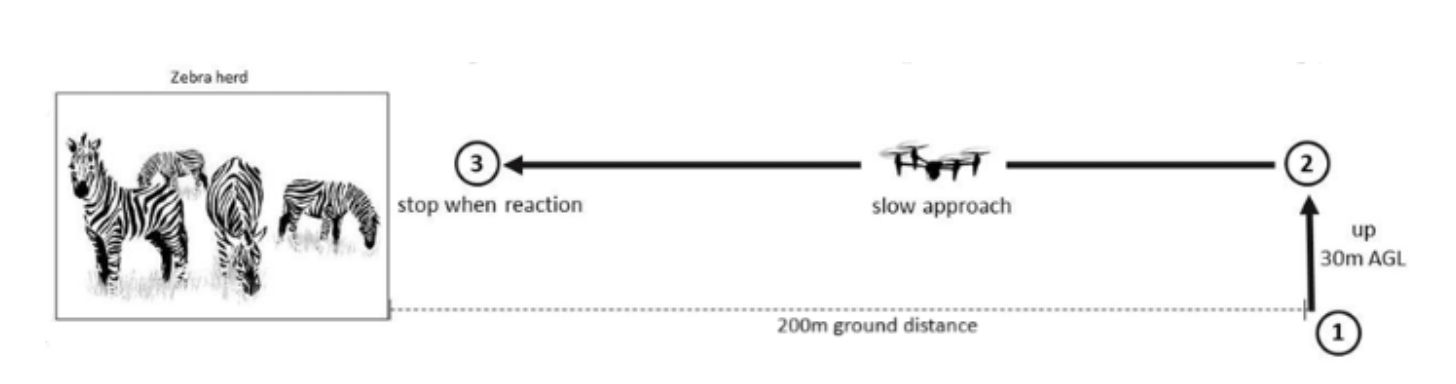
\includegraphics[width=\textwidth]{figures/wv1.png}
        \caption{Horizontal approach at 30m AGL}
        \label{fig:subfig1}
    \end{subfigure}
    \hfill
    \begin{subfigure}[b]{0.45\textwidth}
        \centering
        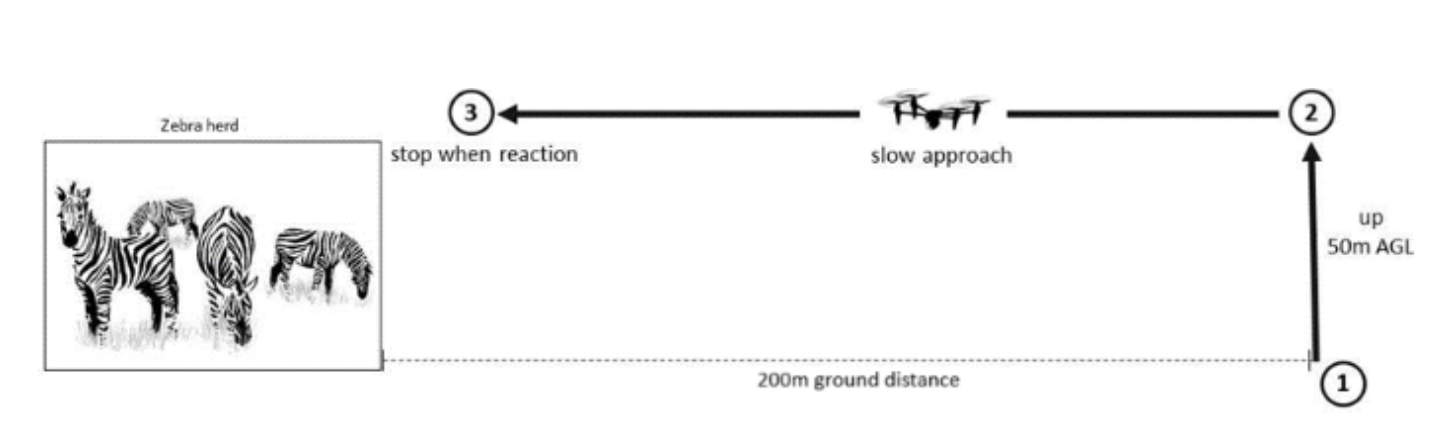
\includegraphics[width=\textwidth]{figures/wv2.png}
        \caption{Horizontal approach at 50m AGL}
        \label{fig:subfig2}
    \end{subfigure}
    \hfill
    \begin{subfigure}[b]{0.45\textwidth}
        \centering
        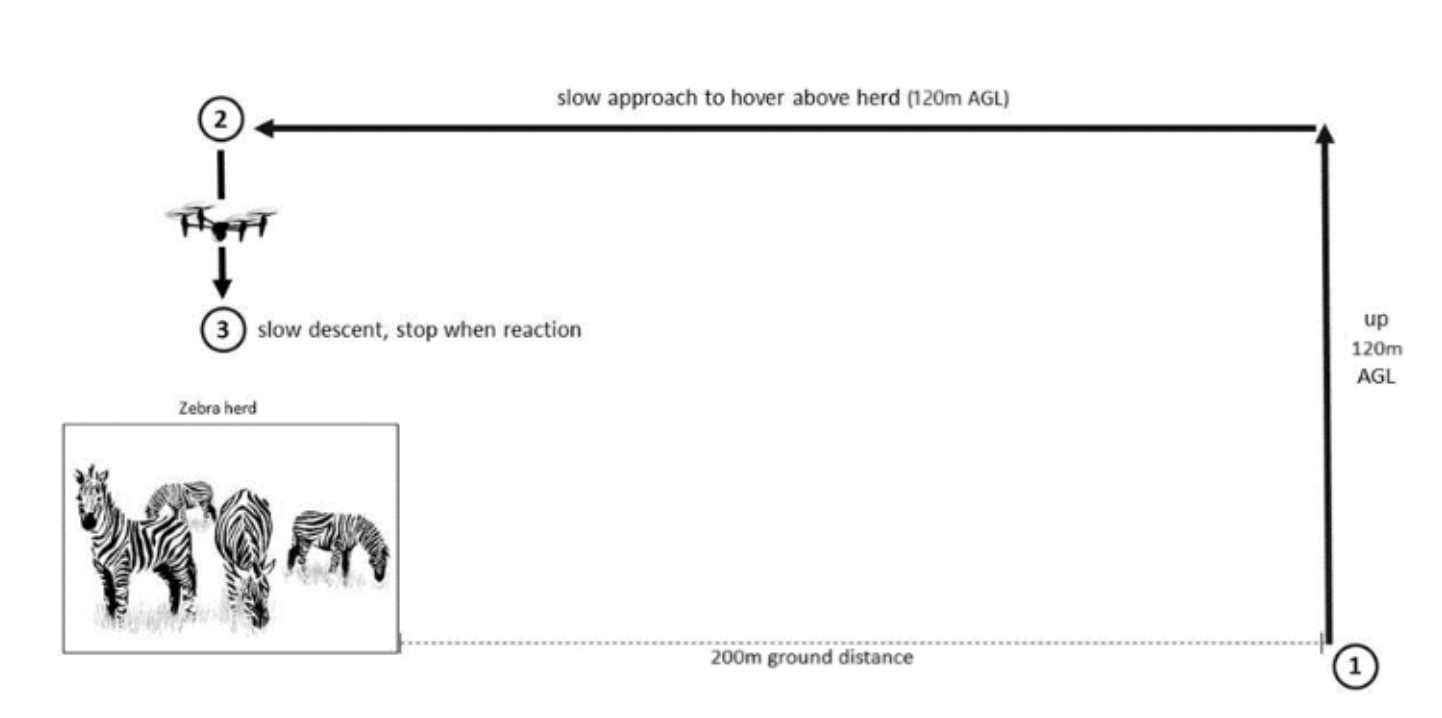
\includegraphics[width=\textwidth]{figures/wv3.png}
        \caption{Vertical approach at 120m AGL}
        \label{fig:subfig3}
    \end{subfigure}
    \caption{Wild Vigilance Animal Approaches}
    \label{fig:drone_approaches}
\end{figure}

\subsubsection{Equipment}
\begin{itemize}
    \item Drone DJI Mavic 3 Thermal Drone
    \item G.R.A.S Microphone array
    \item Hand-held camera
    \item Binoculars
    \item Night-vision rangefinder
    \item Ethograms/observation sheets
\end{itemize}


\subsection{WildWing Protocol}
The human pilot will orient the drone facing the target animals, and the drone will be launched.
The WildDrone system will autonomously launch the drone deploying the horizontal approach at 30m AGL.
The drone will move toward the target animals, until the object detector detects the animals.
The system will be tested in different habitats and at different times of day.
We will also test updated YOLO models for object detection and tracking in the field.
We will test on a variety of herd sizes to test the system's resiliency in the face of large groups of animals,
especially fusion-fission of subgroups within the herd.

\subsubsection{Equipment}
\begin{itemize}
    \item 2 Parrot Anafi Drones
    \item GPU enabled laptop
    \item Hand-held camera
    \item Binoculars
    \item Ethograms/observation sheets
\end{itemize}

\subsubsection{Software}
New WildWing software will be tested in the field. The software has three main screens: 
Launch, Monitoring, and Data Analysis, illustrated in 
\cref{fig:fig1}, \cref{fig:fig2}, and \cref{fig:fig3}.
The software will be used to record zebra behavior autonomously using drones in the field.

\begin{figure}
    \centering
    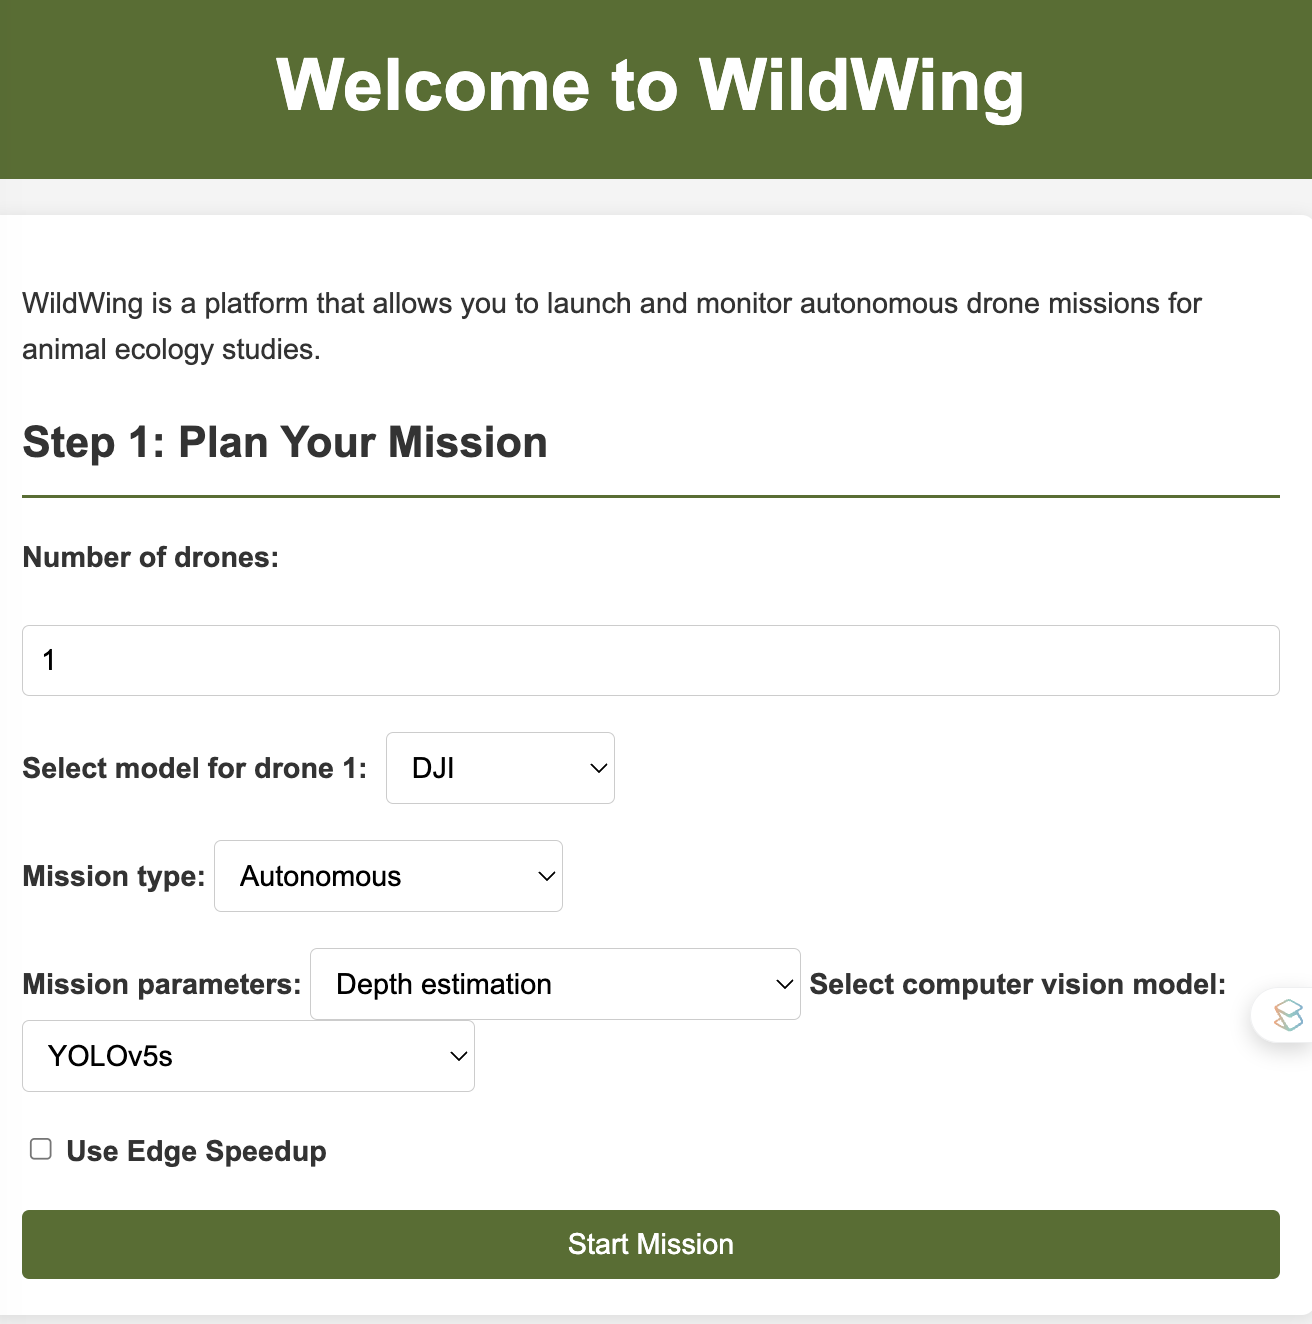
\includegraphics[width=0.45\textwidth]{figures/ww3.png}
    \caption{Launch Screen}
    \label{fig:fig1}
\end{figure}

\begin{figure}
    \centering
    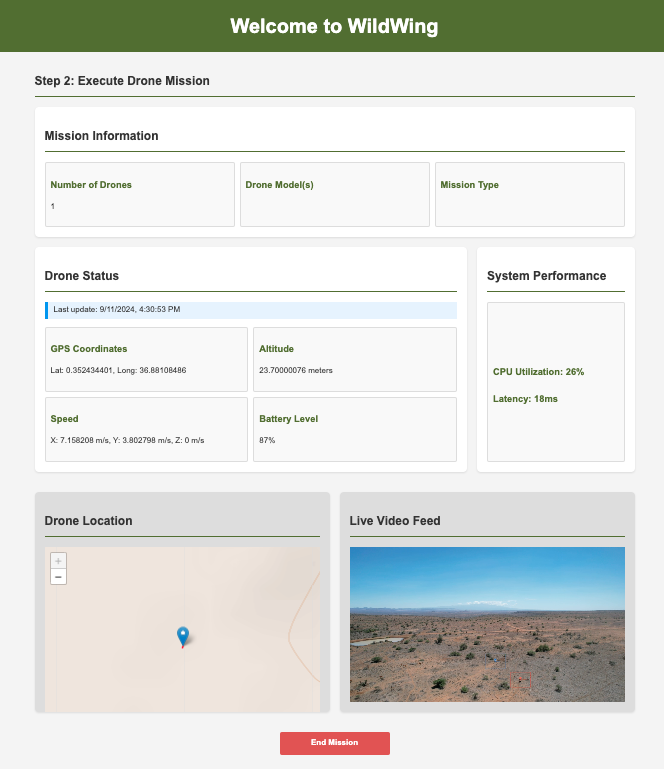
\includegraphics[width=0.45\textwidth]{figures/ww1.png}
    \caption{Monitoring Screen}
    \label{fig:fig2}
\end{figure}

\begin{figure}
    \centering
    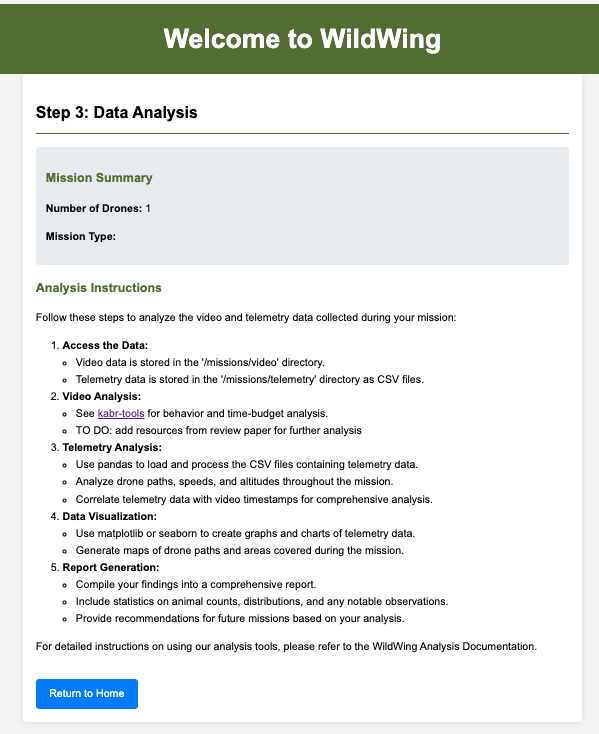
\includegraphics[width=0.45\textwidth]{figures/ww2.png}
     \caption{Data Analysis Screen}
    \label{fig:fig3}
\end{figure}


\section{Relevance}
% Explain why this research question is significant in the context of the course theme.
The WildDroneEU project aims to develop a drone-based system for wildlife monitoring that is both effective and non-invasive.
This project is significant because it will provide valuable data on how drone noise impacts wildlife vigilance 
in different habitats and at different times of day.
This data will help us understand how drones can be used to monitor wildlife without causing undue stress to the animals.
The WildWing project will test an autonomous system for wildlife monitoring using drones in the field.
This system has the potential to revolutionize the way we monitor wildlife populations and track their movements.
By combining the data collected from the WildVigilance and WildWing projects, we will be able to gain a better 
understanding of how drones can be used to monitor wildlife in a way that is both effective and ethical.



\end{document}